\documentclass[a4paper,10pt,twocolumn]{scrartcl}

\usepackage[left=1.5cm,right=1.5cm,top=2.5cm,bottom=2.5cm]{geometry}

\usepackage[utf8]{inputenc}
\usepackage[T1]{fontenc}
\usepackage{hyphenat}
\usepackage{graphicx}
\usepackage{xcolor}
\usepackage[skip=0pt]{caption}
\usepackage[hidelinks]{hyperref}


% set some spacings manually (to avoid big vertical whitspace in columns)
\RedeclareSectionCommand[beforeskip=2ex ,afterskip=1ex]{section}
\RedeclareSectionCommand[beforeskip=1ex]{subsection}
\setparsizes{0pt}{0.5ex}{0pt plus 1fil}
\setlength{\textfloatsep}{1ex}
\setlength{\intextsep}{1ex}



\author{Frank Ebel 01429282, Josef Glas 08606876\\Felix Korbelius 01526132, Johannes Schabbauer 11776224}
\title{\vspace*{-1cm}Management Summary DOPP Exercise 3}
\subtitle{Group 10, Question 20}
\date{\today \vspace*{-0.8cm}}




\begin{document}
\sffamily
\maketitle

This is the Management Summary of the third exercise for the lecture \emph{Data-oriented Programming Paradigms} (188.995).  From the task question 20 was chosen by our group. The work was done equally by all collaborators of group 10 mentioned above. The aim of this document is to present the task, approach and findings of the investigations in a simple manner.

\section{Topic}

The goal of our data-science topic was to investigate the \emph{use of nuclear energy}, where the work was divided into three sections:

First, we show how the constitution of different types of electricity production has evolved over time and how the output of nuclear reactors changed in countries. Next, it was investigated if there if any connection between changes of greenhouse gas emissions and the usage of nuclear energy. In the third section, possible correlations of nuclear energy production with further characteristics of countries, like population or economical and political indicators were investigated.

\section{Approach}

For the key part of the data, which is the production of electricity in nations worldwide, there were two sources accessible: from the \emph{U.S. Energy Information Administration} (USEIA) and \emph{BP}. In a comparison of those to each other no discrepancies were found and we decided to use the USEIA dataset in the further analysis. 
The number of operating nuclear reactors were retrieved from the public section of PRIS (Power Reactor Information System) from the IAEA (International Atomic Energy Agency).

Our investigation includes all available nations worldwide, in the time interval from 1980 to 2018. However, due the emergence of new countries (e.g. from the breakup of the USSR) and very sparse availability of some information at the beginning of this time interval, many comparisons only include the 20 years from 1998 to 2018. 

\section{Findings}

\subsection{How has the use of nuclear energy evolved over time?}

In Fig.~\ref{fig:q1_plot1} the evolution of electricity production is shown. One can see that from 1980 to 2018, the total output worldwide doubled. The amount of nuclear energy in the constitution did not change dramatically. Although the produced nuclear energy more than doubled between 1980 and 2018, from 2000 there was almost no increase and it dropped after the Fukushima disaster in 2011.

\begin{figure}[h]
	\centering
 	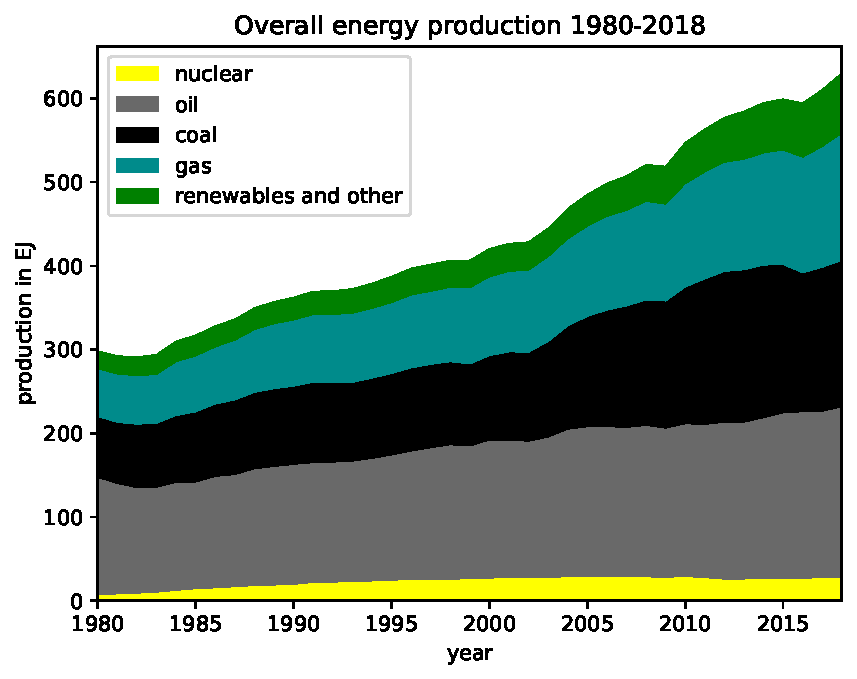
\includegraphics[width=\columnwidth]{../figures/q1_plot1.pdf}
 	\caption{Constitution of worldwide energy production over time.}
 	\label{fig:q1_plot1}
\end{figure}

To compare the change of nuclear usage in different countries, in Fig.~\ref{fig:q2_plot2} the top 20 producers in the year 1998 and 2018 are shown. The largest increase in this time span can be seen for USA, Russia and China, whereas significant drops are observed in Japan, Germany and United Kingdom. One point that can be emphasized is that in the USA and Canada, there was a decrease of operating reactors, but an increase of energy output, which indicates that the size and workload (or efficiency) of their nuclear reactors was in bigger in 2018 than in 1998.

We also want to point out that no import or export of electricity across nation borders could be investigated, because no public database contained information about that. Indeed this would have been very interesting for countries like Austria, that do not produce nuclear energy but depend on import of electric energy.

\begin{figure*}[t]
	\centering
	%\vspace{-1cm} % decrease space in necessary
	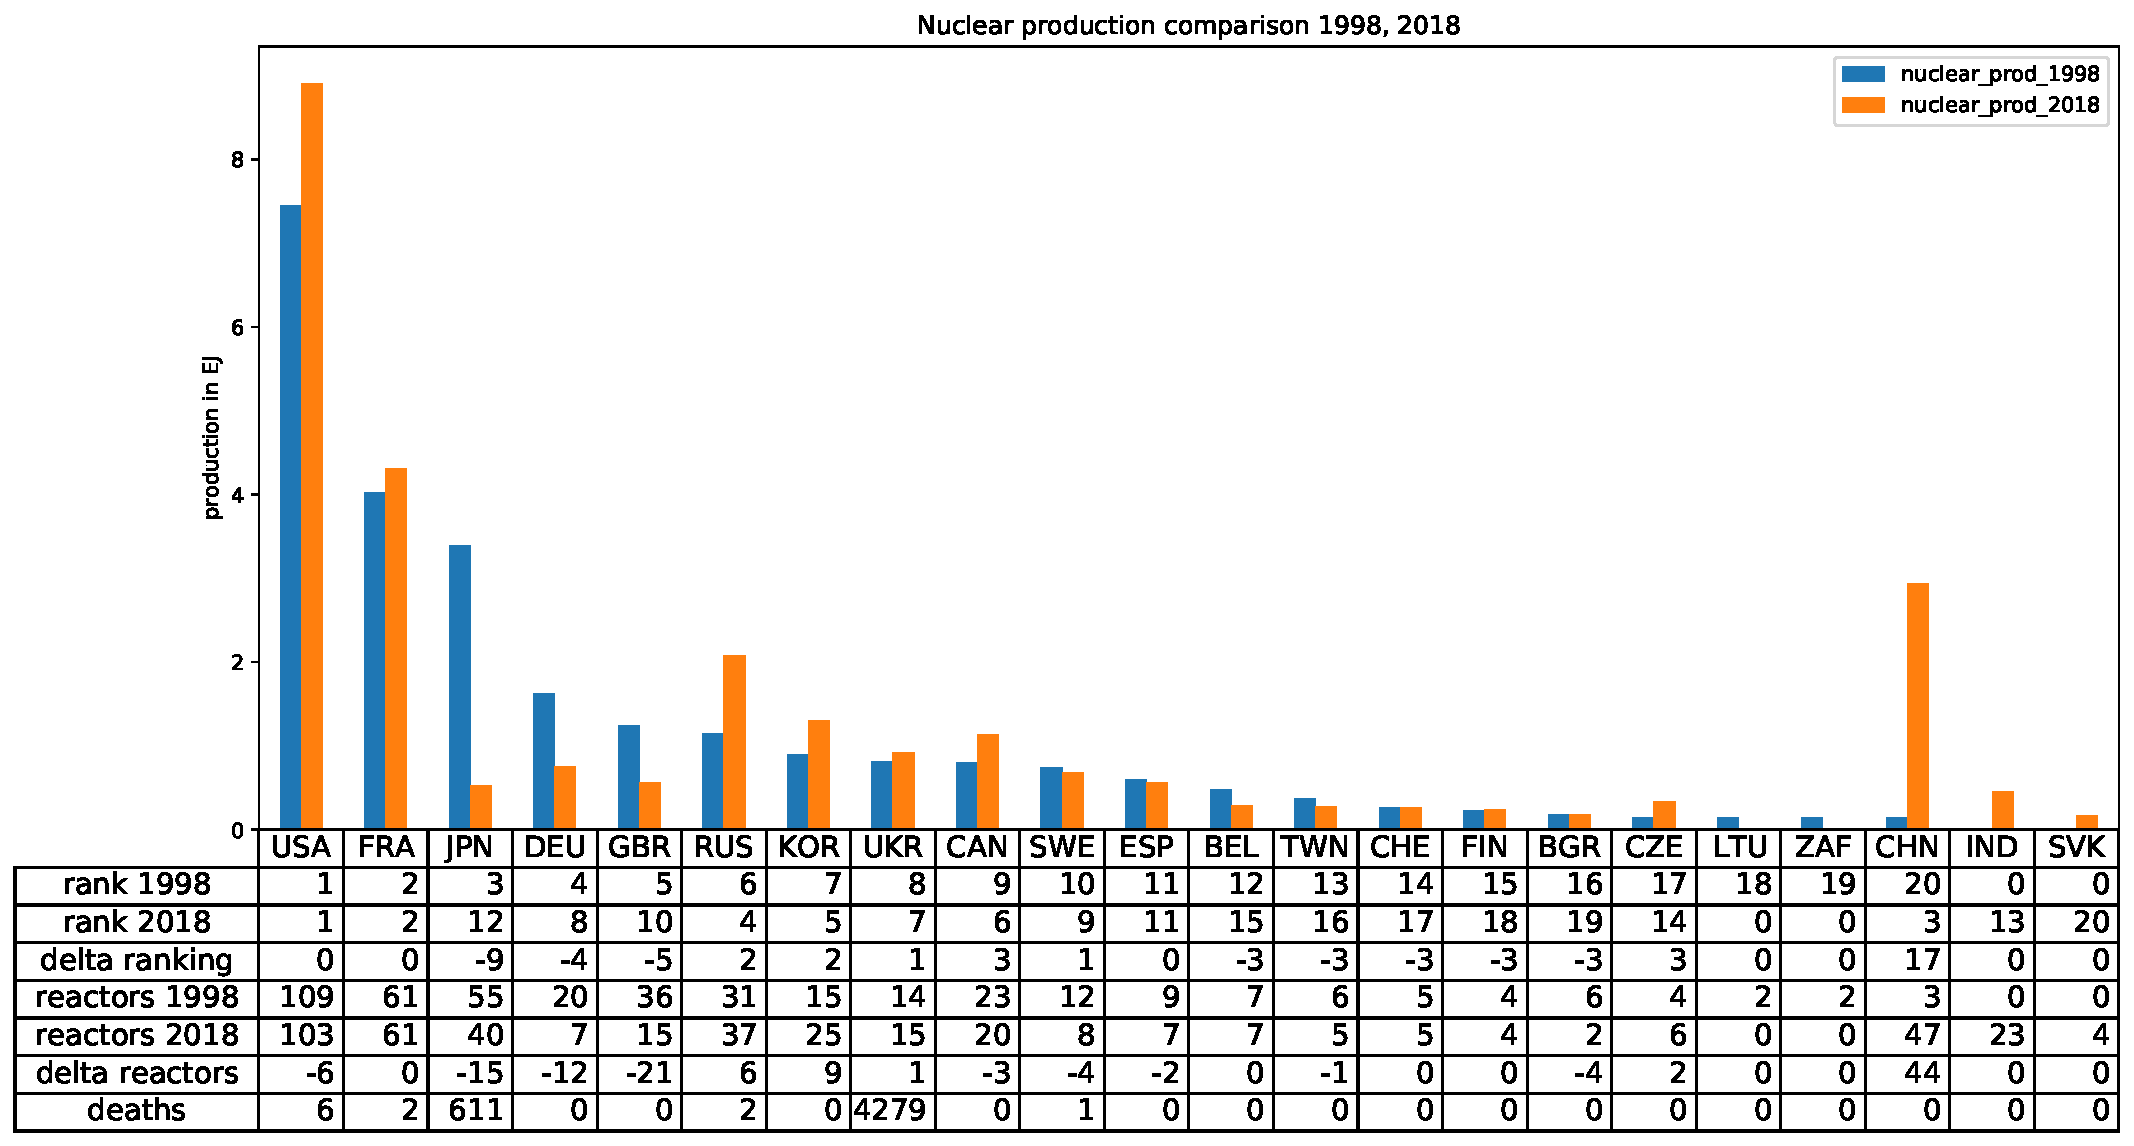
\includegraphics[width=0.8\textwidth]{../figures/q1_plot2.pdf}
	\caption{Largest producers of nuclear energy in 1998, compared to their produced nuclear energy in 2018.}
	\label{fig:q2_plot2}
\end{figure*}

\subsection{How well does the use of nuclear energy correlate with changes in carbon emissions?}



\subsection{Are there characteristics of a country that correlate with increases or decreases in the use of nuclear energy?}

The first property of nations that do or do not use nuclear energy that was investigated, was their population. The result, Fig.~\ref{fig:q3_population}, shows that since China started its first nuclear reactor in 1991, more than half of the worlds population lives in a country with active use of nuclear energy. The number of countries, however, that use nuclear energy is constant at about 30 from more than 200 nations worldwide. Although this graph does not show anything about the \emph{change of nuclear energy usage} because of the simple yes/no classification, it reveals that mostly large countries produce electricity by nuclear fission.

\begin{figure}[hbt]
	\centering
	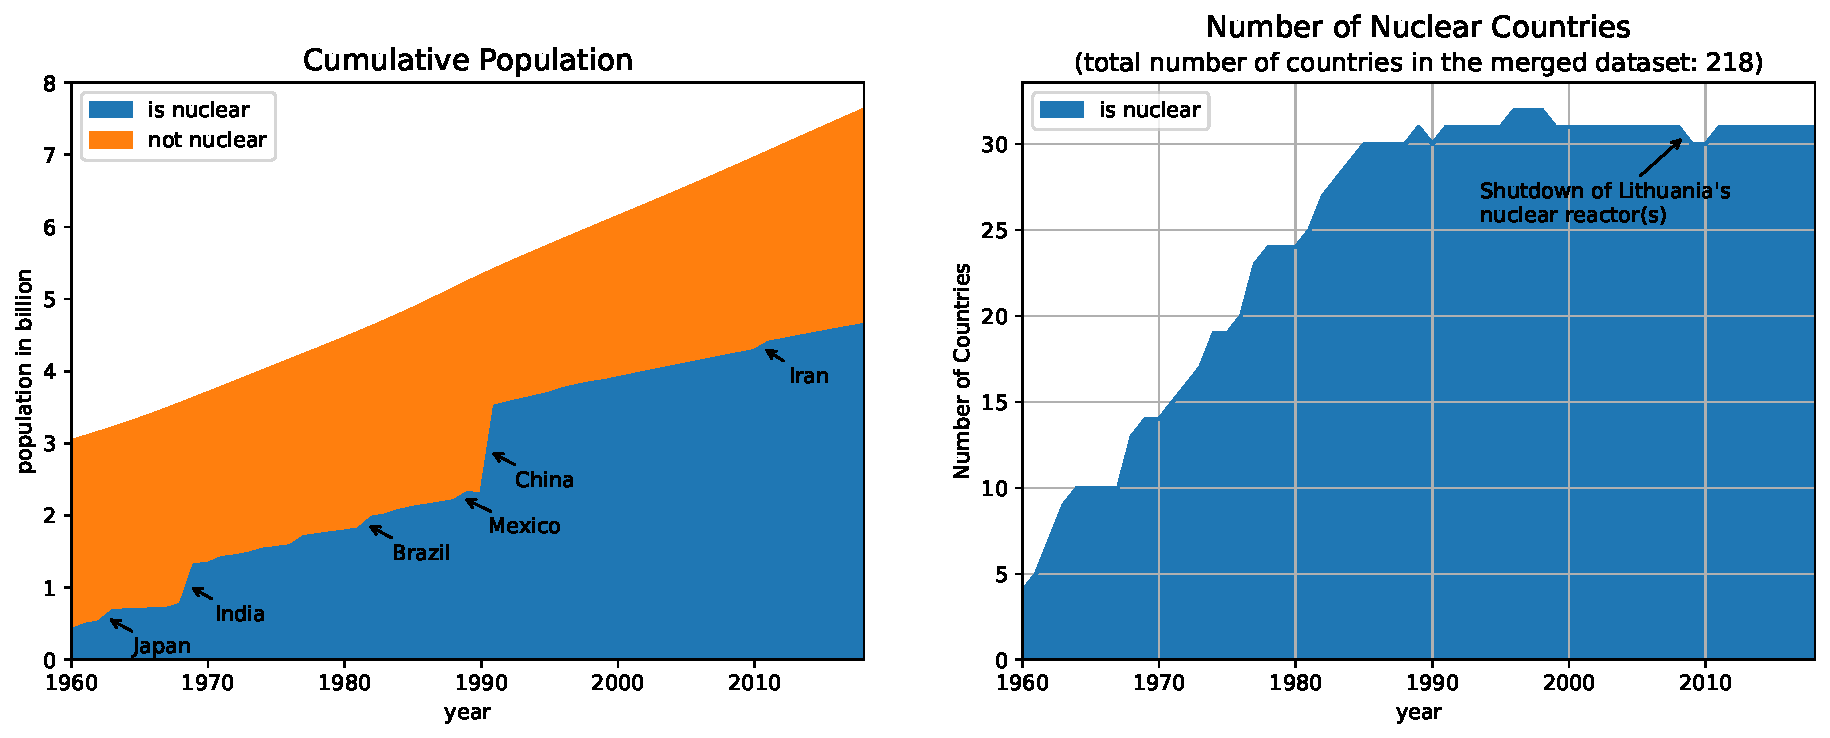
\includegraphics[width=\columnwidth, trim=0 0 160mm 0, clip]{../figures/q3_population.pdf}
	\caption{Change of worldwide population, split into countries that do or do not produce nuclear energy.}
	\label{fig:q3_population}
\end{figure}

Further investigation was done by comparing the relative change of the nuclear energy production between 1998 and 2018 for each country to those of population, GDP (per capita), income (per capita), research expenditure, number of nuclear warheads and five democracy indices from the IDEA (International Institute for Democracy and Electoral Assistance): representative government, fundamental rights, checks on government, impartial administration and civil society participation. Unfortunately, no absolute correlations can be seen between these these indicators and nuclear usage, but by looking at single countries some interesting insight can be gained (see interactive plot in notebook).

\end{document}
